% !TeX root = ../main.tex
\section{V2：以过程一致性为中心的可追溯工作流}
\label{sec:v2}
\subsection{研究思路}
V2 首先处理实际科学计算中过程与证据的一致性问题。其基本组织方式是将已知计算协议分解为明确步骤，在受控启动、状态保存和产物关联的基础上形成可复核计算链。模型决策并非这一阶段量化成果的主要来源；研究重点在于确认计算确实发生、原始结果得到保留，并能够在不重算的情况下恢复其科学含义。

这一设计对应自主计算的基础要求：若输入几何、实际执行条件或输出来源不能被可靠识别，即使后续加入语言模型，也难以判断模型所使用的数值是否属于正确任务。因此，V2 将真实执行与离线科学重解析分离，以固定结果验证证据保存和解释的一致性。

\subsection{计算结果}
本文采用两条人工逐节点批准的成功计算链作为 V2 案例。水和乙醇均使用 ORCA 6.1.1、气相、零电荷、单重态及 r$^{2}$SCAN-3c/TightSCF，执行优化、频率和单点计算。r$^{2}$SCAN-3c 是具有组合校正的复合电子结构方法\cite{r2scan3c}。后续科学分析读取已有输出，没有启动重复计算。结果见表 \ref{tab:v2} 和图 \ref{fig:v2-convergence}。

\begin{table}[htbp]
\centering\small
\caption{V2 两条受控计算链的结果。耗时为 ORCA 各节点自报经过时间之和，未包含人工等待及工作流开销；不同分子和核数不用于计算加速比。}
\label{tab:v2}
\begin{tabularx}{\linewidth}{p{5.3cm}YY}
\toprule
指标 & 水 H$_2$O & 乙醇 C$_2$H$_6$O\\
\midrule
核数 / 总内存 / MaxCore & 1 / 2048 MB / 1536 MB & 4 / 2048 MB / 384 MB\\
成功计算节点 & Opt、Freq、SP 各一次 & Opt、Freq、SP 各一次\\
优化周期 & 4 & 11\\
优化末次评价电子能 / $\Eh$ & $-76.418938721015$ & $-155.002314096955$\\
后续单点电子能 / $\Eh$ & $-76.418938721035$ & $-155.002314094574$\\
首周期至优化终态降能 / m$\Eh$ & 1.692636839 & 7.859199377\\
正振动模式数 & 3 & 21\\
正频率范围 / cm$^{-1}$ & 1653.249--3932.735 & 248.134--3837.522\\
三节点自报总耗时 / s & 24.143 & 98.855\\
\bottomrule
\end{tabularx}
\end{table}

\begin{figure}[htbp]
\centering
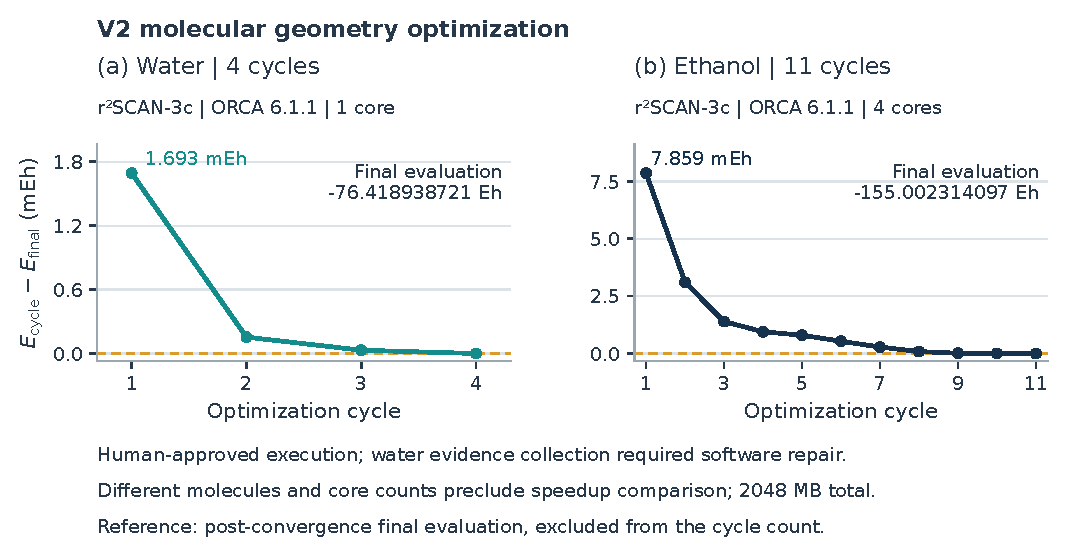
\includegraphics[width=\linewidth]{v2-optimization.pdf}
\caption{V2 水与乙醇的优化收敛曲线。纵轴为各周期电子能减去对应优化末次评价能量，单位 m$\Eh$。收敛后的末次评价仅提供零点，不额外计作优化周期。}
\label{fig:v2-convergence}
\end{figure}

水与乙醇分别获得 3、21 个正振动模式，历史检查支持其给定理论水平下的局部极小值。定义 $\Delta E=E_{\mathrm{SP}}-E_{\mathrm{Opt,final}}$，两者的内部重复评价差分别为 $-2.0\times10^{-11}\,\Eh$ 与 $2.381\times10^{-9}\,\Eh$。该差值反映同一终态的数值一致性，而非相对实验或高精度参考的误差。

\subsection{方法边界与后续问题}
上述成果建立了实际计算与证据复核的可行性，但不构成无人干预的成功率估计：两条链经过人工批准，水链的结果采集还包含开发者修正。单一初始构型也不能支持全局构象结论。V2 因此提供的是可靠操作与可复核证据的基础，而尚未检验自然语言需求如何自主转化为组合计算。后者构成 V3 的主要研究问题。
